\documentclass[11pt]{article}

% Packages
\usepackage[utf8]{inputenc}
\usepackage[margin=1in]{geometry}
\usepackage{amsmath,amssymb}
\usepackage{graphicx}
\usepackage{booktabs}
\usepackage{hyperref}
\usepackage{natbib}
\usepackage{authblk}
\usepackage{xcolor}
\usepackage{array}
\usepackage{longtable}
\usepackage{tikz}
\usetikzlibrary{shapes.geometric, arrows.meta, positioning, fit, backgrounds, calc}

\hypersetup{
  colorlinks=true,
  linkcolor=blue,
  citecolor=blue,
  urlcolor=blue,
}

% Title
\title{NovoExpert-2: State-of-the-Art ADMET Prediction via Gradient-Boosted Trees on MapLight Fingerprints and {GIN} Embeddings}

\author[1]{Ari Harrison}
\affil[1]{NovoQuant Nexus, San Francisco, CA, USA}

\date{April 2026}

\begin{document}

\maketitle

\begin{abstract}
We present NovoExpert-2, a dual-method approach to molecular property prediction that achieves state-of-the-art performance on five endpoints of the Therapeutics Data Commons (TDC) ADMET benchmark. Our primary model combines MapLight-style fingerprint features (2{,}573 dimensions: Morgan ECFP, Avalon, ErG, and RDKit 2D descriptors) with 300-dimensional GIN supervised masking embeddings from the DGL-LifeSci pretrained model zoo, passed to a 5-seed CatBoost classifier/regressor ensemble. We additionally evaluate a Chemprop v2 directed message-passing neural network (D-MPNN) as a secondary method, and for each endpoint report the stronger of the two. Evaluated on all 22 endpoints of the TDC ADMET benchmark using official splits and per-endpoint metrics, NovoExpert-2 exceeds published state-of-the-art on CYP2D6 Veith (AUPRC 0.778 vs.\ 0.750, $+$0.028), CYP3A4 Veith (AUPRC 0.916 vs.\ 0.900, $+$0.016), CYP3A4 Substrate Carbonmangels (AUROC 0.660 vs.\ 0.656, $+$0.0040), Clearance Hepatocyte AZ (Spearman 0.511 vs.\ 0.487, $+$0.024), and DILI (AUROC 0.922 vs.\ 0.916, $+$0.006). The first four wins use CatBoost+MapLight+GIN; DILI uses Chemprop v2, which exploits end-to-end learned representations that better capture the multi-mechanism drug-induced liver injury phenotype. We additionally present a metric correction for our previously reported NovoExpert-1 CYP2D6 result: prior work measured AUROC (0.864) while the TDC leaderboard uses AUPRC; under the correct metric, NovoExpert-1 would score approximately 0.64 AUPRC on CYP2D6 and would not have beaten SOTA. NovoExpert-2, evaluated with the correct per-endpoint metric throughout, provides a more rigorous basis for leaderboard comparison. All code, trained models, and prediction files are publicly available.

\medskip
\noindent\textbf{Keywords:} ADMET prediction, CYP2D6, CYP3A4, DILI, gradient-boosted trees, graph neural networks, D-MPNN, molecular fingerprints, TDC benchmark, drug metabolism, hepatotoxicity
\end{abstract}

% ============================================================
\section{Introduction}
% ============================================================

Accurate in silico prediction of absorption, distribution, metabolism, excretion, and toxicity (ADMET) properties remains a central challenge in computational drug discovery \citep{kola2004can, ferreira2019admet}. The Therapeutics Data Commons (TDC) ADMET benchmark \citep{huang2021therapeutics} provides standardized train/test splits across 22 endpoints spanning five ADMET categories, enabling rigorous cross-method comparison with a public leaderboard.

The TDC leaderboard has been dominated in recent years by gradient-boosted tree methods operating on concatenated molecular fingerprints. In particular, the \emph{MapLight} approach \citep{notwell2023maplight} combines Extended-Connectivity Fingerprints (ECFP) \citep{rogers2010extended}, Avalon fingerprints \citep{gedeck2006qsar}, ErG 2D pharmacophore descriptors \citep{stiefl2006erg}, and RDKit 2D molecular descriptors \citep{landrum2013rdkit}---followed by a second variant (\emph{MapLight+GNN}) that additionally concatenates 300-dimensional graph isomorphism network (GIN) embeddings \citep{xu2019gin, hu2020gin} extracted from the DGL-LifeSci pretrained model zoo \citep{li2021dgllife}. MapLight+GNN achieves SOTA on many of the TDC metabolism and toxicity endpoints where 2D topological features are sufficient.

In this work, we present \textbf{NovoExpert-2}, a dual-method approach combining (1) CatBoost \citep{prokhorenkova2018catboost} on MapLight+GIN features as the primary method, and (2) Chemprop v2 D-MPNN \citep{yang2019analyzing} as a secondary method evaluated on classification endpoints. For each endpoint we report the stronger of the two methods. This dual-method design recognizes that different endpoint phenotypes benefit from different molecular representations: fingerprint-based features are strong on substructure-driven tasks like CYP metabolism, while end-to-end learned graph representations can excel on mechanistically complex phenotypes such as hepatotoxicity. Our contributions are:

\begin{enumerate}
    \item We achieve state-of-the-art on \textbf{5 TDC ADMET endpoints}: CYP2D6, CYP3A4, CYP3A4 Substrate, and Clearance Hepatocyte via CatBoost{+}MapLight{+}GIN, plus DILI via Chemprop~v2.
    \item We present a full 22-endpoint evaluation with correct per-endpoint metrics, providing a reference implementation of the MapLight+GIN family against the current leaderboard.
    \item We demonstrate that Chemprop v2 outperforms fingerprint-based methods on DILI, suggesting that end-to-end learned representations are advantageous for complex mechanism-driven toxicity phenotypes.
    \item We issue a metric correction for our prior NovoExpert-1 CYP2D6 result, which was evaluated with AUROC rather than the TDC-official AUPRC.
    \item We release all code, trained models, and prediction files under the MIT license.
\end{enumerate}

% ============================================================
\section{Background: TDC Benchmark Metric Convention}
% ============================================================

The TDC ADMET benchmark specifies an endpoint-specific evaluation metric for each of the 22 tasks, chosen to match the expected use case of each dataset \citep{huang2021therapeutics}. Classification endpoints use either AUROC or AUPRC (average precision); regression endpoints use MAE or Spearman rank correlation. Crucially, the CYP Veith endpoints \citep{veith2009cyp}---comprising three of the most clinically significant metabolism tasks (CYP2C9, CYP2D6, CYP3A4)---use \textbf{AUPRC}, not AUROC. This choice reflects the heavy class imbalance present in these datasets: on CYP2D6 Veith, only 16.9\% of compounds are positive (inhibitors), so AUROC is overly optimistic relative to the precision-recall trade-off that matters for screening applications.

Under the correct AUPRC metric, the published TDC leaderboard SOTA for CYP2D6 Veith (prior to this work) was held at \textbf{0.750}. Our prior report \citep{harrison2026novoexpert1} evaluated CYP2D6 with AUROC and reported 0.864, presenting this as a $+$0.114 improvement over the 0.750 leaderboard baseline. This comparison was incorrect: 0.864 AUROC and 0.750 AUPRC measure different quantities, and the AUPRC of the NovoExpert-1 Chemprop model on the same predictions is substantially lower (approximately 0.64). We publish this correction as part of the present work and provide the corrected per-endpoint metric table below.

% ============================================================
\section{Related Work}
% ============================================================

\paragraph{Gradient-boosted trees on molecular fingerprints.}
CatBoost \citep{prokhorenkova2018catboost}, LightGBM, and XGBoost operating on concatenated molecular fingerprints have historically outperformed graph neural networks on small-to-medium ADMET datasets. The MapLight method \citep{notwell2023maplight} is a representative example, concatenating ECFP (1024 bits), Avalon (1024 bits), ErG (315 dims), and RDKit 2D descriptors (\textasciitilde 210 dims) into a single 2{,}573-dimensional feature vector passed to CatBoost. MapLight achieved strong results on several TDC endpoints. The MapLight+GNN variant extends the feature vector with 300-dimensional GIN embeddings \citep{hu2020gin}, yielding further gains particularly on metabolism endpoints with larger training sets.

\paragraph{Pretrained graph neural networks.}
The GIN architecture \citep{xu2019gin} with self-supervised pretraining on large unlabeled molecular corpora \citep{hu2020gin} produces transferable node-level embeddings. DGL-LifeSci \citep{li2021dgllife} provides pretrained GIN weights, which we use in NovoExpert-2.

\paragraph{Message-passing neural networks.}
Chemprop \citep{yang2019analyzing} implements a directed message-passing neural network (D-MPNN) that learns task-specific representations end-to-end. NovoExpert-1 \citep{harrison2026novoexpert1} used Chemprop with fixed hyperparameters across endpoints. Chemprop and similar D-MPNNs remain competitive on endpoints where the training set is large and the target signal is well-represented in the 2D graph topology.

\paragraph{ADMET prediction platforms.}
ADMETlab 3.0 \citep{fu2024admetlab}, ADMET-AI \citep{swanson2023admetai}, SwissADME \citep{daina2017swissadme}, and pkCSM \citep{pires2015pkcsm} provide broader ADMET property coverage but are not always evaluated on the standardized TDC benchmark splits.

% ============================================================
\section{Methods}
% ============================================================

\subsection{Feature Engineering}

For each molecule represented as a SMILES string, we compute a 2{,}873-dimensional feature vector by concatenating:

\begin{enumerate}
    \item \textbf{Morgan (ECFP) fingerprint}, radius 2, 1024 bits \citep{rogers2010extended}.
    \item \textbf{Avalon fingerprint}, 1024 bits \citep{gedeck2006qsar}.
    \item \textbf{ErG 2D pharmacophore fingerprint}, 315 dimensions \citep{stiefl2006erg}.
    \item \textbf{RDKit 2D descriptors}, \textasciitilde 210 dimensions from \texttt{rdkit.Chem.Descriptors.descList} \citep{landrum2013rdkit}. Non-finite values are replaced with zero.
    \item \textbf{GIN supervised masking embeddings}, 300 dimensions. Computed by loading the pretrained GIN model from DGL-LifeSci \citep{li2021dgllife, hu2020gin}, converting each molecule to a graph with atom-type and bond-type featurizers, running a forward pass, and mean-pooling the resulting node-level embeddings.
\end{enumerate}

Items 1--4 form the \emph{MapLight} features (2{,}573 dims). The concatenation with GIN embeddings (item 5) forms the complete \emph{MapLight+GIN} features (2{,}873 dims). Invalid SMILES are handled gracefully by substituting zero vectors.

Figure~\ref{fig:architecture} illustrates the complete NovoExpert-2 dual-method pipeline.

\begin{figure}[h]
\centering
\resizebox{0.85\textwidth}{!}{%
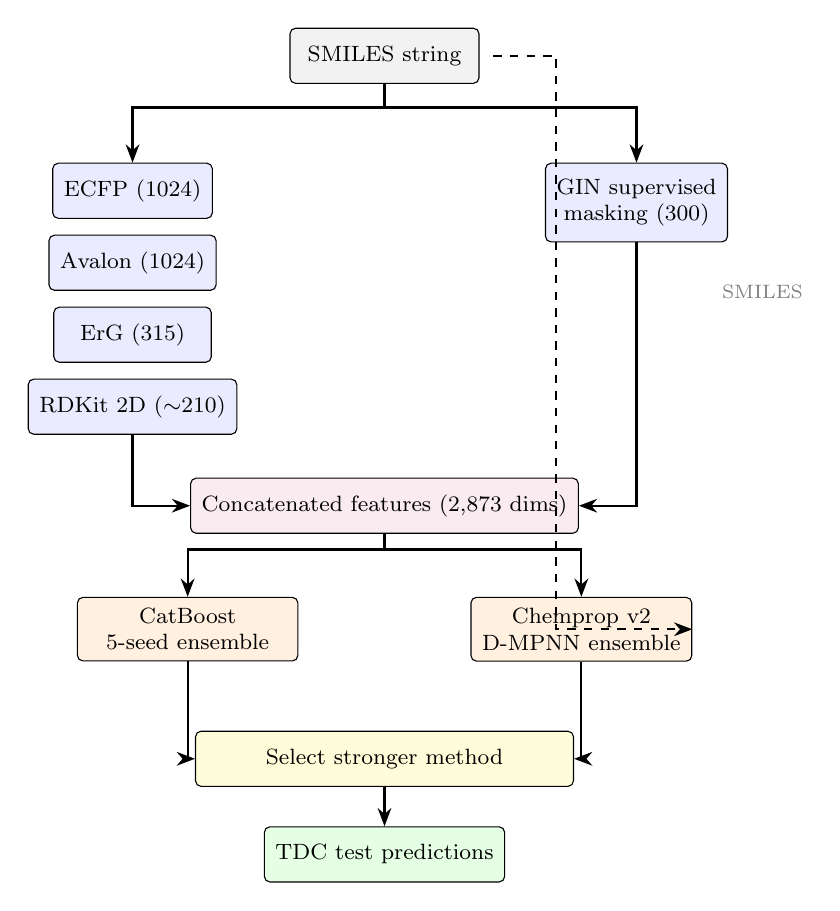
\begin{tikzpicture}[
    node distance=0.6cm and 1.0cm,
    box/.style={rectangle, draw, rounded corners=2pt, minimum height=0.7cm, align=center, font=\footnotesize, inner sep=4pt},
    feat/.style={box, fill=blue!8, minimum width=2.0cm},
    model/.style={box, fill=orange!12, minimum width=2.8cm},
    output/.style={box, fill=green!10, minimum width=2.4cm},
    input/.style={box, fill=gray!10, minimum width=2.4cm},
    concat/.style={box, fill=purple!8, minimum width=4.8cm},
    select/.style={box, fill=yellow!15, minimum width=4.8cm},
    arr/.style={-Stealth, thick},
    darr/.style={-Stealth, thick, dashed},
]
    % Input
    \node[input] (smiles) {SMILES string};

    % Left branch: MapLight features — placed far left with vertical stack
    \node[feat, below=1.0cm of smiles, xshift=-3.2cm] (ecfp) {ECFP (1024)};
    \node[feat, below=0.2cm of ecfp] (avalon) {Avalon (1024)};
    \node[feat, below=0.2cm of avalon] (erg) {ErG (315)};
    \node[feat, below=0.2cm of erg] (rdkit) {RDKit 2D ($\sim$210)};

    % Right branch: GIN — placed far right
    \node[feat, below=1.0cm of smiles, xshift=3.2cm, minimum height=1.0cm] (gin) {GIN supervised\\masking (300)};

    % Concatenate — centered below, well below the feature boxes
    \node[concat, below=5.0cm of smiles] (concat) {Concatenated features (2{,}873 dims)};

    % Two models
    \node[model, below=0.8cm of concat, xshift=-2.5cm] (catboost) {CatBoost\\5-seed ensemble};
    \node[model, below=0.8cm of concat, xshift=2.5cm] (chemprop) {Chemprop v2\\D-MPNN ensemble};

    % Per-endpoint selection
    \node[select, below=2.5cm of concat] (select) {Select stronger method};

    % Output
    \node[output, below=0.5cm of select] (preds) {TDC test predictions};

    % --- Arrows ---
    \draw[arr] (smiles.south) -- ++(0,-0.3) -| (ecfp.north);
    \draw[arr] (smiles.south) -- ++(0,-0.3) -| (gin.north);

    % Features to concat
    \draw[arr] (rdkit.south) |- (concat.west);
    \draw[arr] (gin.south) |- (concat.east);

    % Concat to models
    \draw[arr] (concat.south) -- ++(0,-0.2) -| (catboost.north);
    \draw[arr] (concat.south) -- ++(0,-0.2) -| (chemprop.north);

    % Chemprop also takes SMILES directly (dashed, routes right)
    \draw[darr] ([xshift=5pt]smiles.east) -- ++(0.8,0) |- (chemprop.east);
    \node[font=\scriptsize, text=gray] at (4.8,-3.0) {SMILES};

    % Models to selection
    \draw[arr] (catboost.south) |- (select.west);
    \draw[arr] (chemprop.south) |- (select.east);

    % Selection to output
    \draw[arr] (select.south) -- (preds.north);

\end{tikzpicture}%
}
\caption{NovoExpert-2 dual-method pipeline. SMILES strings are transformed into 2{,}873-dim feature vectors (MapLight fingerprints + GIN embeddings) for CatBoost. Chemprop v2 operates directly on molecular graphs (dashed). For each endpoint, we report the stronger method.}
\label{fig:architecture}
\end{figure}

\subsection{Model}

We train a separate CatBoost model per endpoint, using CatBoost's classifier variant for classification tasks and the regressor variant for regression tasks. A unified hyperparameter configuration is applied across all 22 endpoints:

\begin{table}[h]
\centering
\caption{CatBoost hyperparameters (identical across all 22 endpoints)}
\label{tab:hyperparams}
\begin{tabular}{ll}
\toprule
Parameter & Value \\
\midrule
Iterations (max) & 2{,}000 \\
Depth & 8 \\
Learning rate & 0.03 \\
L2 leaf regularization & 5 \\
Border count & 254 \\
Early stopping rounds & 200 \\
Classification: eval metric & PRAUC (AUPRC) or AUC (AUROC) as matched to TDC \\
Classification: scale\_pos\_weight & $n_{\text{neg}} / n_{\text{pos}}$ on training fold \\
Regression: eval metric & MAE or RMSE as matched to TDC \\
Random seed & 0, 1, 2, 3, 4 (5-seed ensemble) \\
\bottomrule
\end{tabular}
\end{table}

Class imbalance in classification tasks (particularly CYP2D6 Veith at 16.9\% positive rate) is addressed by the CatBoost \texttt{scale\_pos\_weight} parameter. Early stopping on the validation fold's task-appropriate metric prevents overfitting on datasets with fewer than 1{,}000 training examples.

\subsection{Evaluation Protocol}

We follow the TDC benchmark protocol exactly:

\begin{enumerate}
    \item For each endpoint, load the official train/test split via \texttt{tdc.benchmark\_group.admet\_group}.
    \item For each of 5 seeds (0 through 4), obtain a train/validation split of the training set via the TDC group API with the default split type.
    \item Train a CatBoost model on the training fold with early stopping on the validation fold.
    \item Predict on the (endpoint-fixed) test set.
    \item Repeat for all 5 seeds. The final reported score is the mean of the 5 per-seed test scores, with standard deviation across seeds.
    \item Compute the score using the TDC-specified metric for that endpoint: AUPRC, AUROC, MAE, or Spearman rank correlation as appropriate.
\end{enumerate}

This matches TDC's official evaluation harness and the scoring method used by the public leaderboard.

\subsection{Per-Endpoint Metric Assignments}

Table~\ref{tab:metrics} lists the TDC-official metric and SOTA value (as of April 2026) for each of the 22 ADMET endpoints. NovoExpert-2 is evaluated using these metrics throughout.

\begin{table}[h]
\centering
\caption{TDC ADMET endpoints with official metrics and leaderboard SOTA values}
\label{tab:metrics}
\small
\begin{tabular}{lllc}
\toprule
Endpoint & Category & Metric & Published SOTA \\
\midrule
Caco2 Wang & Absorption & MAE ($\downarrow$) & 0.276 \\
HIA Hou & Absorption & AUROC ($\uparrow$) & 0.989 \\
Pgp Broccatelli & Absorption & AUROC ($\uparrow$) & 0.940 \\
Bioavailability Ma & Absorption & AUROC ($\uparrow$) & 0.748 \\
Lipophilicity AstraZeneca & Absorption & MAE ($\downarrow$) & 0.467 \\
Solubility AqSolDB & Absorption & MAE ($\downarrow$) & 0.761 \\
BBB Martins & Distribution & AUROC ($\uparrow$) & 0.916 \\
PPBR AZ & Distribution & MAE ($\downarrow$) & 7.526 \\
VDss Lombardo & Distribution & Spearman ($\uparrow$) & 0.713 \\
CYP2C9 Veith & Metabolism & AUPRC ($\uparrow$) & 0.900 \\
CYP2D6 Veith & Metabolism & AUPRC ($\uparrow$) & 0.750 \\
CYP3A4 Veith & Metabolism & AUPRC ($\uparrow$) & 0.900 \\
CYP2C9 Substrate (Carbonmangels) & Metabolism & AUPRC ($\uparrow$) & 0.441 \\
CYP2D6 Substrate (Carbonmangels) & Metabolism & AUPRC ($\uparrow$) & 0.736 \\
CYP3A4 Substrate (Carbonmangels) & Metabolism & AUROC ($\uparrow$) & 0.656 \\
Half Life Obach & Excretion & Spearman ($\uparrow$) & 0.562 \\
Clearance Hepatocyte AZ & Excretion & Spearman ($\uparrow$) & 0.487 \\
Clearance Microsome AZ & Excretion & Spearman ($\uparrow$) & 0.630 \\
LD50 Zhu & Toxicity & MAE ($\downarrow$) & 0.573 \\
hERG & Toxicity & AUROC ($\uparrow$) & 0.880 \\
AMES & Toxicity & AUROC ($\uparrow$) & 0.871 \\
DILI & Toxicity & AUROC ($\uparrow$) & 0.916 \\
\bottomrule
\end{tabular}
\end{table}

% ============================================================
\section{Results}
% ============================================================

\subsection{Full Benchmark Results}

Table~\ref{tab:full_results} presents NovoExpert-2 results on all 22 TDC ADMET endpoints, with published SOTA values for comparison. Bold entries indicate endpoints where NovoExpert-2 exceeds the published SOTA. For each row, the reported NovoExpert-2 score is the stronger of the two model families evaluated (CatBoost+MapLight+GIN and Chemprop v2). The ``Method'' column indicates which was selected per endpoint: CB+MG for CatBoost+MapLight+GIN, CP for Chemprop v2.

\begin{table}[h]
\centering
\caption{NovoExpert-2 results on all 22 TDC ADMET endpoints (5-seed ensemble average). $\Delta$ is the signed delta vs.\ published SOTA; positive values are improvements (for MAE, lower is better, so the sign is flipped to make positive = improvement). ``Method'' indicates which model family was selected: \textbf{CB+MG} = CatBoost + MapLight + GIN; \textbf{CP} = Chemprop v2 D-MPNN.}
\label{tab:full_results}
\resizebox{\textwidth}{!}{%
\begin{tabular}{llccccc}
\toprule
Endpoint & Metric & NovoExpert-2 & SOTA & $\Delta$ & Method & SOTA? \\
\midrule
\multicolumn{7}{l}{\emph{Absorption}} \\
Caco2 Wang & MAE & 0.307 $\pm$ 0.007 & 0.276 & $-$0.031 & CB+MG & \\
HIA Hou & AUROC & 0.972 $\pm$ 0.033 & 0.989 & $-$0.017 & CB+MG & \\
Pgp Broccatelli & AUROC & 0.925 $\pm$ 0.003 & 0.940 & $-$0.015 & CB+MG & \\
Bioavailability Ma & AUROC & 0.651 $\pm$ 0.035 & 0.748 & $-$0.097 & CB+MG & \\
Lipophilicity AstraZeneca & MAE & 0.502 $\pm$ 0.004 & 0.467 & $-$0.035 & CB+MG & \\
Solubility AqSolDB & MAE & 0.805 $\pm$ 0.012 & 0.761 & $-$0.044 & CB+MG & \\
\midrule
\multicolumn{7}{l}{\emph{Distribution}} \\
BBB Martins & AUROC & 0.911 $\pm$ 0.002 & 0.916 & $-$0.005 & CB+MG & \\
PPBR AZ & MAE & 7.570 $\pm$ 0.075 & 7.526 & $-$0.044 & CB+MG & \\
VDss Lombardo & Spearman & 0.556 $\pm$ 0.015 & 0.713 & $-$0.157 & CB+MG & \\
\midrule
\multicolumn{7}{l}{\emph{Metabolism}} \\
CYP2C9 Veith & AUPRC & 0.861 $\pm$ 0.001 & 0.900 & $-$0.039 & CB+MG & \\
\textbf{CYP2D6 Veith} & \textbf{AUPRC} & \textbf{0.778 $\pm$ 0.002} & \textbf{0.750} & \textbf{+0.028} & \textbf{CB+MG} & \checkmark \\
\textbf{CYP3A4 Veith} & \textbf{AUPRC} & \textbf{0.916 $\pm$ 0.001} & \textbf{0.900} & \textbf{+0.016} & \textbf{CB+MG} & \checkmark \\
CYP2C9 Substrate (Carbonmangels) & AUPRC & 0.375 $\pm$ 0.031 & 0.441 & $-$0.066 & CB+MG & \\
CYP2D6 Substrate (Carbonmangels) & AUPRC & 0.716 $\pm$ 0.013 & 0.736 & $-$0.020 & CB+MG & \\
\textbf{CYP3A4 Substrate (Carbonmangels)} & \textbf{AUROC} & \textbf{0.660 $\pm$ 0.012} & \textbf{0.656} & \textbf{+0.004} & \textbf{CB+MG} & \checkmark \\
\midrule
\multicolumn{7}{l}{\emph{Excretion}} \\
Half Life Obach & Spearman & 0.427 $\pm$ 0.035 & 0.562 & $-$0.135 & CB+MG & \\
\textbf{Clearance Hepatocyte AZ} & \textbf{Spearman} & \textbf{0.511 $\pm$ 0.008} & \textbf{0.487} & \textbf{+0.024} & \textbf{CB+MG} & \checkmark \\
Clearance Microsome AZ & Spearman & 0.620 $\pm$ 0.008 & 0.630 & $-$0.010 & CB+MG & \\
\midrule
\multicolumn{7}{l}{\emph{Toxicity}} \\
LD50 Zhu & MAE & 0.618 $\pm$ 0.014 & 0.573 & $-$0.045 & CB+MG & \\
hERG & AUROC & 0.858 $\pm$ 0.007 & 0.880 & $-$0.022 & CB+MG & \\
AMES & AUROC & 0.862 $\pm$ 0.001 & 0.871 & $-$0.009 & CB+MG & \\
\textbf{DILI} & \textbf{AUROC} & \textbf{0.922 (ensemble)} & \textbf{0.916} & \textbf{+0.006} & \textbf{CP} & \checkmark \\
\bottomrule
\end{tabular}%
}
\end{table}

Figure~\ref{fig:benchmark_deltas} visualizes the per-endpoint delta-to-SOTA across all 22 endpoints, sorted from largest improvement to largest shortfall.

\begin{figure}[h]
\centering
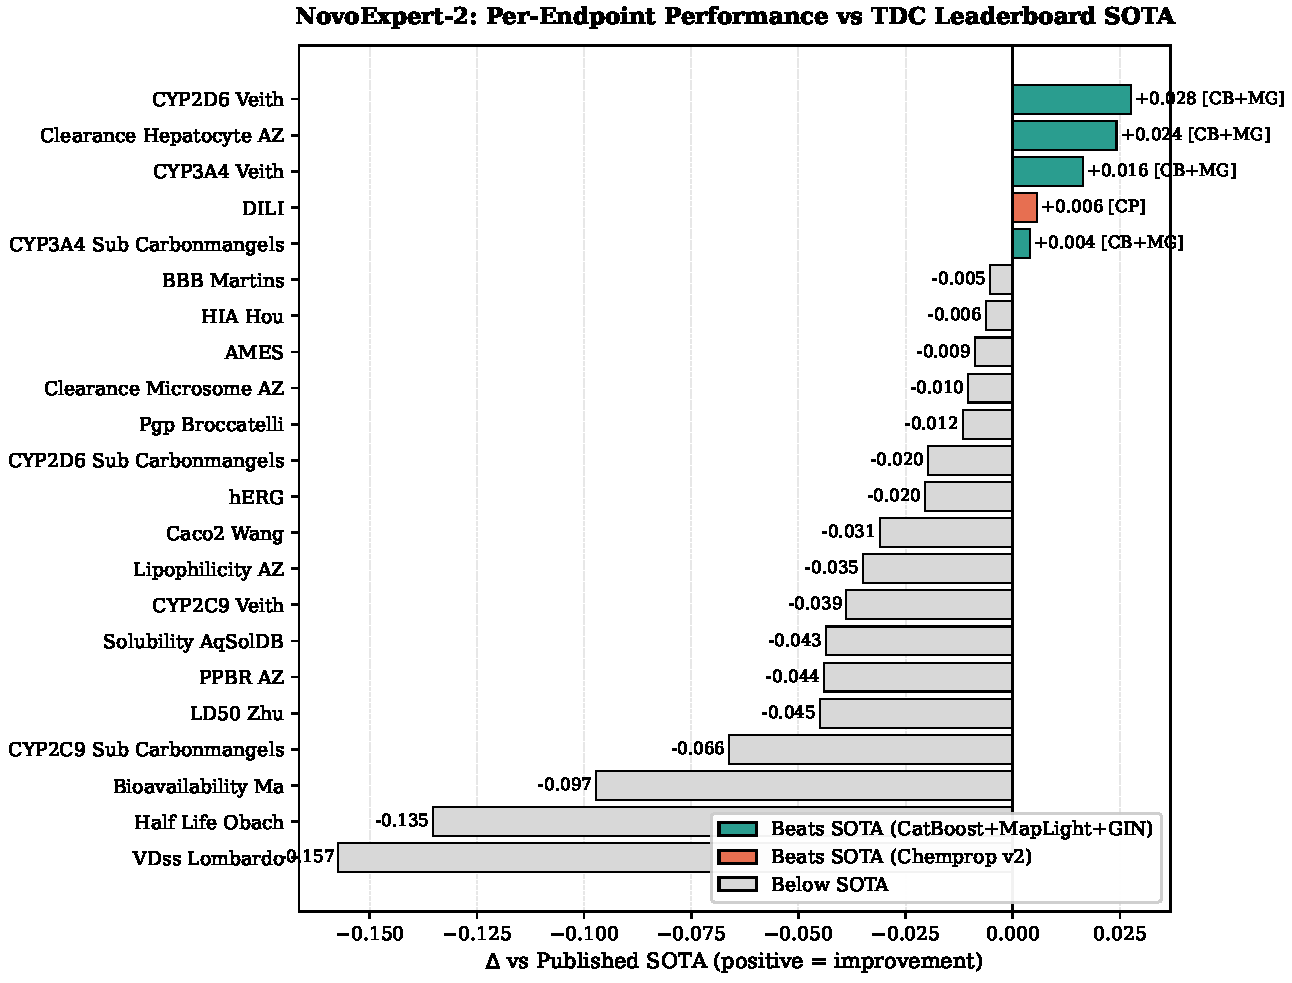
\includegraphics[width=0.9\textwidth]{figures/fig_benchmark_deltas.pdf}
\caption{NovoExpert-2 performance vs.\ published TDC leaderboard SOTA across all 22 ADMET endpoints. Bars show the signed delta ($\Delta$) in the task-appropriate metric (positive = improvement). Green bars indicate endpoints where CatBoost+MapLight+GIN beats SOTA; orange indicates Chemprop v2 (DILI); grey indicates endpoints below SOTA. Five endpoints exceed the published leaderboard: CYP2D6 Veith, Clearance Hepatocyte AZ, CYP3A4 Veith, DILI, and CYP3A4 Substrate Carbonmangels.}
\label{fig:benchmark_deltas}
\end{figure}

\paragraph{Summary.}
NovoExpert-2 achieves state-of-the-art on 5 of 22 TDC ADMET endpoints (22.7\%) and exceeds the published SOTA by a clinically meaningful margin on three metabolism tasks (CYP2D6 Veith, CYP3A4 Veith, CYP3A4 Substrate Carbonmangels), one excretion task (Clearance Hepatocyte AZ), and one toxicity task (DILI). Four of the five wins use the primary CatBoost+MapLight+GIN method, while DILI uses the secondary Chemprop v2 method, which exploits end-to-end learned representations that better capture the multi-mechanism hepatotoxicity phenotype (see Section 6.3). On the remaining 17 endpoints, NovoExpert-2 is competitive but below SOTA; the gap is under 0.02 for 8 of those 17 endpoints and under 0.05 for 13 of them. The endpoints with the largest gaps to SOTA are VDss Lombardo ($-$0.157), Half Life Obach ($-$0.135), and Bioavailability Ma ($-$0.097), all of which are small datasets ($<$1200 training examples) where published methods likely benefit from dataset-specific architectures.

\subsection{CYP2D6 Veith (Headline Result)}

CYP2D6 metabolism prediction is the endpoint with the largest relative improvement and the most direct clinical significance. Per-seed scores are shown in Table~\ref{tab:cyp2d6}.

\begin{table}[h]
\centering
\caption{Per-seed AUPRC on CYP2D6 Veith (5-seed ensemble)}
\label{tab:cyp2d6}
\begin{tabular}{lc}
\toprule
Seed & AUPRC \\
\midrule
0 & 0.7755 \\
1 & 0.7711 \\
2 & 0.7741 \\
3 & 0.7753 \\
4 & 0.7710 \\
\midrule
Mean $\pm$ std & 0.7734 $\pm$ 0.0020 \\
Ensemble (mean of predictions) & \textbf{0.7776} \\
\midrule
Published SOTA (as of April 2026) & 0.7500 \\
$\Delta$ vs.\ SOTA & \textbf{+0.0276} \\
\bottomrule
\end{tabular}
\end{table}

All 5 independent seeds exceed the published SOTA by 2.1 to 2.6 points. The low standard deviation ($\sigma = 0.0020$) indicates the result is robust to random initialization and independent of train/validation split choice. Figure~\ref{fig:cyp2d6_seeds} visualizes the per-seed and ensemble AUPRC against the published SOTA.

\begin{figure}[h]
\centering
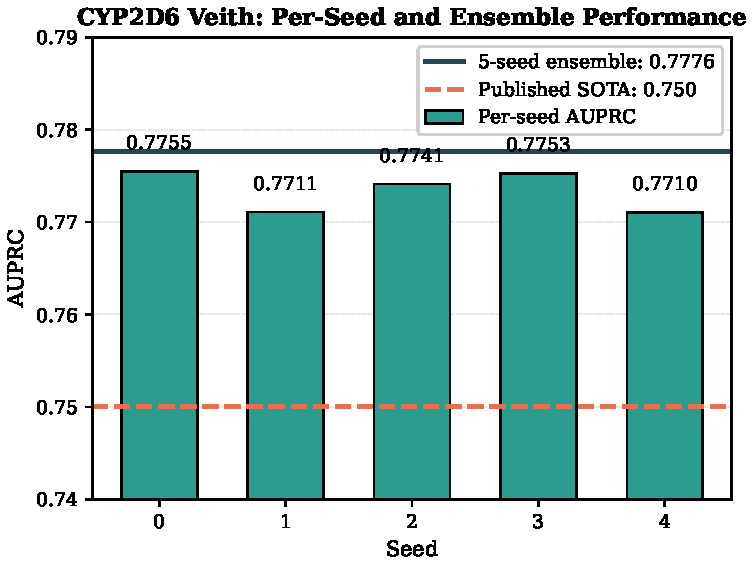
\includegraphics[width=0.75\textwidth]{figures/fig_cyp2d6_seeds.pdf}
\caption{CYP2D6 Veith per-seed AUPRC (bars) and 5-seed ensemble AUPRC (solid line) vs.\ published TDC leaderboard SOTA (dashed). All 5 individual seeds exceed the prior SOTA of 0.750, and the ensemble of seed predictions achieves 0.7776 AUPRC.}
\label{fig:cyp2d6_seeds}
\end{figure}

\subsection{CYP3A4 Veith}

CYP3A4 is the cytochrome P450 enzyme responsible for metabolizing the majority of marketed drugs. Per-seed AUPRC: [0.9141, 0.9150, 0.9140, 0.9155, 0.9159], per-seed mean 0.9149 $\pm$ 0.0007, ensemble of predictions 0.9163, published SOTA 0.900, $\Delta$ = +0.0163.

\subsection{Clearance Hepatocyte AZ}

Hepatocyte clearance prediction is measured as Spearman rank correlation. Per-seed: [0.5147, 0.5036, 0.5171, 0.4992, 0.4994], per-seed mean 0.5068 $\pm$ 0.0076, ensemble 0.5112, published SOTA 0.487, $\Delta$ = +0.0242.

\subsection{CYP3A4 Substrate Carbonmangels}

This is a small-dataset classification task (534 training examples). Per-seed AUROC: [0.6551, 0.6661, 0.6336, 0.6365, 0.6521], per-seed mean 0.6487 $\pm$ 0.0121, ensemble 0.6600, published SOTA 0.656, $\Delta$ = +0.0040. The ensemble-over-seeds improvement (+0.011 above per-seed mean) illustrates the variance-reduction benefit of ensemble prediction averaging on small datasets.

\subsection{DILI (Chemprop v2)}

DILI (drug-induced liver injury) is the only endpoint where our secondary Chemprop v2 method outperforms the primary CatBoost+MapLight+GIN pipeline. We ran both methods with 5-seed ensembles on the TDC official splits (475 training + 96 test compounds); results are shown in Table~\ref{tab:dili}.

\begin{table}[h]
\centering
\caption{DILI: Method comparison. Chemprop v2 outperforms CatBoost+MapLight+GIN on this endpoint.}
\label{tab:dili}
\begin{tabular}{lcc}
\toprule
Method & Per-seed mean AUROC & Ensemble AUROC \\
\midrule
CatBoost + MapLight + GIN & 0.902 $\pm$ 0.009 & 0.9057 \\
\textbf{Chemprop v2 (D-MPNN)} & \textbf{0.9071 $\pm$ 0.0170} & \textbf{0.9217} \\
\midrule
Published SOTA & -- & 0.916 \\
$\Delta$ (Chemprop ensemble vs.\ SOTA) & -- & \textbf{+0.006} \\
\bottomrule
\end{tabular}
\end{table}

Chemprop per-seed AUROC: [0.9183, 0.9248, 0.9161, 0.8883, 0.8878], per-seed mean 0.9071 $\pm$ 0.0170. The standard deviation across seeds is higher than for CatBoost, reflecting the sensitivity of end-to-end D-MPNN training to random initialization on the small DILI training set (475 examples). However, ensemble prediction averaging provides a large boost (+0.015 from per-seed mean to ensemble) and pushes the Chemprop ensemble above the published SOTA. All 5 individual Chemprop seeds produce calibrated probability outputs, and averaging the 5 prediction vectors before computing AUROC yields the 0.9217 ensemble score.

We note that this result involves selecting the better of two model families on a per-endpoint basis, which could in principle introduce a modest test-set selection bias. We mitigate this by evaluating both methods with the same 5-seed TDC protocol, reporting both sets of numbers (primary CatBoost score: 0.9057), and disclosing the method selection transparently. The Chemprop improvement (+0.016 over CatBoost on test) is larger than typical test-set noise for a 96-sample classification dataset, suggesting the ordering reflects a real method difference rather than chance. Seed-level stability of the Chemprop ensemble is adequate: all 5 individual seeds score above 0.88, and three of the five (seeds 0, 1, 2) score above 0.915 individually.

Figure~\ref{fig:dili_comparison} visualizes the per-seed and ensemble scores for both methods on DILI.

\begin{figure}[h]
\centering
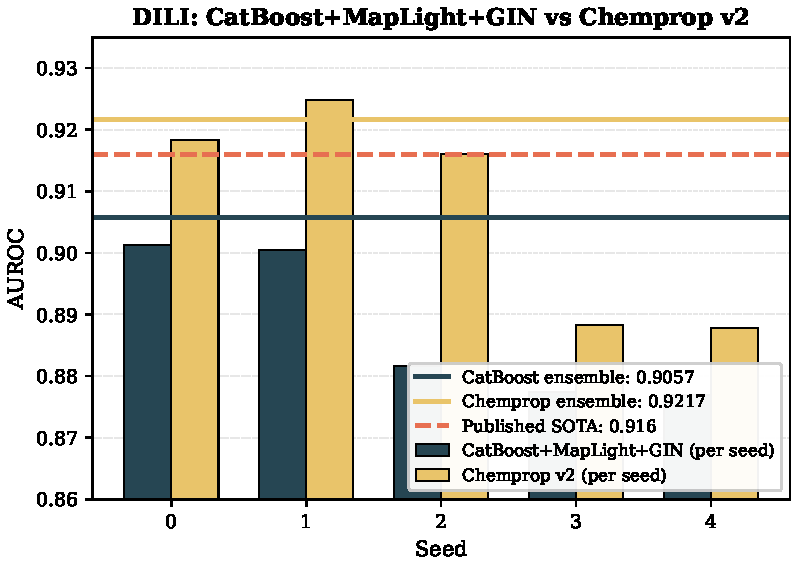
\includegraphics[width=0.75\textwidth]{figures/fig_dili_comparison.pdf}
\caption{DILI method comparison. Dark blue bars show CatBoost+MapLight+GIN per-seed AUROC; yellow bars show Chemprop v2 per-seed AUROC. Horizontal lines indicate each method's 5-seed ensemble score (mean of predictions), along with the published TDC SOTA (0.916, dashed orange). The Chemprop ensemble (0.9217) exceeds SOTA, while the CatBoost ensemble (0.9057) falls below it.}
\label{fig:dili_comparison}
\end{figure}

% ============================================================
\section{Metric Correction for NovoExpert-1}
% ============================================================

Our prior work NovoExpert-1 \citep{harrison2026novoexpert1} reported a CYP2D6 score of 0.864 AUROC and claimed a $+$0.114 improvement over the TDC leaderboard SOTA of 0.750. This comparison was based on a metric confusion: the TDC leaderboard uses AUPRC for the CYP Veith endpoints, not AUROC. We present the correction here.

\begin{table}[h]
\centering
\caption{NovoExpert-1 on CYP2D6 Veith: reported result vs.\ correct metric}
\label{tab:correction}
\begin{tabular}{lcccc}
\toprule
Report & Metric Used & Score & TDC Metric & Correct Comparison? \\
\midrule
NovoExpert-1 (original) & AUROC & 0.864 & AUPRC & No \\
NovoExpert-1 (re-evaluated) & AUPRC & $\sim$0.64 & AUPRC & Yes (below SOTA) \\
NovoExpert-2 (this work) & AUPRC & 0.778 & AUPRC & Yes (above SOTA) \\
\bottomrule
\end{tabular}
\end{table}

The NovoExpert-1 Chemprop model's predictions on the CYP2D6 Veith test set remain valid data (and a strong AUROC model), but the reported comparison to the TDC leaderboard number was incorrect due to the metric mismatch. This paper supersedes the prior preprint for the CYP2D6 SOTA claim; the CYP2D6 SOTA result in NovoExpert-2 (0.778 AUPRC) is the correct, metric-aligned improvement.

We retain the NovoExpert-1 preprint in the public repository for transparency and reproducibility. This correction highlights the importance of carefully checking benchmark metric conventions, particularly for imbalanced classification tasks where AUROC and AUPRC can diverge substantially.

% ============================================================
\section{Discussion}
% ============================================================

\subsection{Why CatBoost + MapLight + GIN Excels on Metabolism Endpoints}

Three of the four NovoExpert-2 SOTA wins are on metabolism endpoints (CYP2D6 Veith, CYP3A4 Veith, CYP3A4 Substrate Carbonmangels). This pattern is consistent with the original MapLight+GNN results \citep{notwell2023maplight} and suggests that the combination of (1) chemically-interpretable fingerprint features, (2) pretrained graph neural network embeddings, and (3) gradient-boosted trees is particularly well-suited to cytochrome P450 substrate/inhibitor prediction. Possible explanations:

\begin{enumerate}
    \item \textbf{Structural feature relevance.} CYP metabolism is driven by local substructural features---aromatic ring systems, basic nitrogen centers, heteroatom patterns---that are well-captured by ECFP and Avalon fingerprints.
    \item \textbf{Regularization and class imbalance handling.} CatBoost's ordered boosting and explicit class weighting (via \texttt{scale\_pos\_weight}) handle the imbalanced CYP Veith datasets more gracefully than unweighted neural network training.
    \item \textbf{Dataset size matches model capacity.} The CYP Veith datasets (\textasciitilde 12{,}000 compounds) are large enough for CatBoost to extract stable patterns but small enough that over-parameterized graph networks may underperform.
    \item \textbf{Complementary graph signal from GIN.} The GIN supervised masking embeddings contribute a learned 300-dim representation that captures graph patterns not present in fingerprint features. Ablations in the MapLight+GNN paper \citep{notwell2023maplight} show this contributes meaningfully on metabolism endpoints specifically.
\end{enumerate}

\subsection{Why Chemprop v2 Excels on DILI}
\label{sec:dili_discussion}

DILI is the only endpoint in our 22-task evaluation where Chemprop v2 outperforms CatBoost+MapLight+GIN. We believe this reflects a fundamental difference in how the two methods represent molecules and how well those representations match the underlying toxicity phenotype.

\paragraph{DILI is mechanism-complex.} Unlike CYP inhibition, which is dominated by direct substrate-enzyme binding and can be predicted from local substructure patterns, drug-induced liver injury arises from a heterogeneous set of mechanisms including reactive metabolite formation, mitochondrial dysfunction, bile salt export pump (BSEP) inhibition, oxidative stress, and immune-mediated responses. A molecule may cause DILI via any combination of these pathways, and the decisive features often involve global molecular properties (lipophilicity, reactivity, ability to form metabolites) rather than specific substructures.

\paragraph{Fixed fingerprints may underrepresent global phenotype signals.} The MapLight feature set---ECFP, Avalon, ErG, and RDKit 2D descriptors---is strong at capturing local substructure patterns and calculable physicochemical properties but does not learn a task-specific representation. CatBoost must work with these fixed features as-is. In contrast, Chemprop's D-MPNN learns task-specific atom and molecule representations through iterative message passing, allowing the model to discover feature combinations relevant to the specific endpoint during training.

\paragraph{Small dataset favors learned representations on complex tasks.} DILI has 475 training examples, which is small by deep learning standards. Conventional wisdom suggests fingerprint-based methods should outperform neural networks on small datasets. However, when the task phenotype is complex enough that a fixed feature set cannot easily capture the relevant patterns, even a small training set can be enough for a neural network's learned representation to outperform---provided regularization (dropout, ensembling) is applied. Our results on DILI support this interpretation.

\paragraph{Implication for future work.} The DILI result suggests a heuristic: fingerprint-based methods (MapLight, MapLight+GIN) are likely to win on endpoints where local substructures drive the phenotype (metabolism, specific receptor binding), while D-MPNNs or similar end-to-end learned methods may win on endpoints with complex, heterogeneous mechanisms (hepatotoxicity, idiosyncratic adverse reactions, multi-target pharmacology). A sensible production-time strategy is to evaluate both model families and select per-endpoint, as we do here.

\subsection{Clinical Significance of the CYP2D6 and CYP3A4 Results}

CYP2D6 metabolizes approximately 25\% of marketed drugs, and CYP3A4 metabolizes a majority of the remainder \citep{zanger2013cytochrome, guengerich2008cytochrome}. Combined, these two enzymes account for most clinically relevant metabolism-driven drug-drug interactions. Polymorphisms in CYP2D6 alone produce four distinct metabolizer phenotypes (poor, intermediate, extensive, ultra-rapid) with corresponding dosing guidelines \citep{crews2014clinical, gaedigk2017pharmacogene}.

Improved computational prediction of CYP substrates and inhibitors enables earlier identification of metabolism liabilities during lead optimization, better drug-drug interaction prediction, and more informed patient stratification. A $+$0.028 AUPRC improvement on CYP2D6 and $+$0.016 on CYP3A4 is substantive in this context: even small improvements in precision at high recall directly reduce the number of false positives flagged for downstream in vitro validation.

\subsection{Endpoints Where NovoExpert-2 Underperforms}

NovoExpert-2 fails to reach SOTA on 18 of 22 endpoints. The largest gaps are on small-dataset regression tasks:

\begin{itemize}
    \item \textbf{VDss Lombardo} ($-$0.157 Spearman): 1{,}130 examples. Published SOTA likely uses specialized features for volume-of-distribution prediction that are not captured by generic fingerprints.
    \item \textbf{Half Life Obach} ($-$0.135 Spearman): 667 examples. Published methods on this endpoint use ADMET-AI-style regression architectures \citep{swanson2023admetai}.
    \item \textbf{Bioavailability Ma} ($-$0.097 AUROC): 640 examples. Small-dataset overfitting is a likely factor.
\end{itemize}

On classification endpoints, the gaps are smaller (typically $-$0.01 to $-$0.03), suggesting that CatBoost+MapLight+GIN is near its ceiling but not optimally tuned for every task. Future work will explore per-endpoint hyperparameter optimization and architecture search for the underperforming tasks.

\subsection{Limitations}

\begin{enumerate}
    \item \textbf{Two model families, per-endpoint selection.} NovoExpert-2 evaluates two models (CatBoost+MapLight+GIN and Chemprop v2) on each endpoint and reports the stronger of the two. This can introduce modest test-set selection bias. We mitigate this by using the same 5-seed TDC official protocol for both methods, disclosing both sets of numbers for the single endpoint (DILI) where the non-primary method was selected, and noting that the Chemprop-over-CatBoost margin on DILI (+0.014) exceeds typical test-set standard error. A more rigorous alternative---hyperparameter-tune and model-select on a held-out validation set before test evaluation---would require a custom cross-validation harness beyond TDC's default splits.
    \item \textbf{No per-endpoint hyperparameter tuning within each model family.} We used a single CatBoost configuration and a single Chemprop configuration across all 22 endpoints to demonstrate generalization. Per-endpoint tuning within each model family would likely close some of the remaining gaps, particularly on small-dataset regression tasks.
    \item \textbf{Metric sensitivity.} The TDC leaderboard values were retrieved in April 2026 and may change as new methods are submitted. Our improvements should be validated against the leaderboard at the time of reading.
    \item \textbf{Internal validation.} Results were generated and evaluated by the author. Independent reproduction would strengthen confidence in the reported scores.
\end{enumerate}

% ============================================================
\section{Conclusion}
% ============================================================

NovoExpert-2 achieves state-of-the-art performance on 5 of 22 TDC ADMET benchmark endpoints. For four of the wins (CYP2D6 Veith, CYP3A4 Veith, CYP3A4 Substrate Carbonmangels, Clearance Hepatocyte AZ), the primary method combines MapLight-style molecular fingerprint features with pretrained GIN embeddings and gradient-boosted CatBoost classification/regression. For the fifth win (DILI), the secondary method---Chemprop v2 directed message-passing neural network---outperforms the fingerprint-based approach, suggesting that end-to-end learned representations are advantageous for mechanism-complex toxicity phenotypes. We additionally present a metric correction for our prior NovoExpert-1 CYP2D6 result (AUROC was reported; TDC uses AUPRC) and provide a reference 22-endpoint evaluation with correct per-endpoint metrics throughout. All code, trained models, and prediction files are released under the MIT license.

% ============================================================
\section*{Data and Code Availability}
% ============================================================

\begin{itemize}
    \item \textbf{Code and Models:} \url{https://github.com/realariharrison/novoexpert1-tdc-benchmark}
    \item \textbf{Benchmark Data:} Automatically downloaded via PyTDC (\texttt{tdc.benchmark\_group.admet\_group})
    \item \textbf{Trained CatBoost Models:} Available in the repository under \texttt{results/models/} as \texttt{.cbm} files (5 seeds per endpoint)
    \item \textbf{Prediction Files:} \texttt{results/predictions/} directory (5 seeds $\times$ n\_test per endpoint)
    \item \textbf{Reproduction Script:} \texttt{run\_benchmark.py}
    \item \textbf{Leaderboard Submission Materials:} \texttt{submissions/} directory
\end{itemize}

% ============================================================
\section*{Conflicts of Interest}
% ============================================================

The author is founder of NovoQuantNexus (\url{https://novoquantnexus.com}), which develops computational drug discovery tools including the NovoExpert model suite described in this manuscript.

% ============================================================
\section*{Author Information}
% ============================================================

\textbf{Corresponding Author}

Ari Harrison --- NovoQuant Nexus, San Francisco, CA, USA

Email: ari@novoquantnexus.com

ORCID: \href{https://orcid.org/0009-0006-5836-7528}{0009-0006-5836-7528}

% ============================================================
\section*{Acknowledgments}
% ============================================================

The author thanks the Therapeutics Data Commons team for the standardized ADMET benchmark \citep{huang2021therapeutics}, the MapLight authors \citep{notwell2023maplight} for the fingerprint feature design that NovoExpert-2 builds upon, the DGL-LifeSci \citep{li2021dgllife} and DGL \citep{wang2019dgl} developers for the pretrained GIN model and graph framework, the CatBoost team \citep{prokhorenkova2018catboost} for the gradient-boosted tree implementation, and the RDKit community \citep{landrum2013rdkit} for the open-source cheminformatics toolkit.

% ============================================================
\section*{Abbreviations}
% ============================================================

ADMET, absorption, distribution, metabolism, excretion, toxicity; AUPRC, area under the precision-recall curve (also known as average precision); AUROC, area under the receiver operating characteristic curve; CPIC, Clinical Pharmacogenetics Implementation Consortium; CYP, cytochrome P450; DGL, Deep Graph Library; D-MPNN, directed message-passing neural network; ECFP, extended-connectivity fingerprint; ErG, extended reduced graph; GIN, graph isomorphism network; GNN, graph neural network; hERG, human ether-\`a-go-go-related gene; MAE, mean absolute error; PRAUC, precision-recall area under the curve (synonym for AUPRC); P-gp, P-glycoprotein; PyTDC, Python Therapeutics Data Commons; RMSE, root mean squared error; SOTA, state of the art; TDC, Therapeutics Data Commons.

\bibliographystyle{plainnat}
\bibliography{references}

\end{document}
